%%
%% static_code_analysis_in_ci.tex
%% V0.1
%% 2015/01/22
%% by 
%% Sebastian Funke
%% Hamza Zulfiqar
%% Brian Pfretzschner
%% See:
%% https://github.com/hzulfiqar/SecSoftDev
%% for current contact information.
%%


\documentclass[conference]{IEEEtran}


% *** PACKAGES ***
%\usepackage{algorithmic}
%\usepackage{array}
%\usepackage{mdwmath}
%\usepackage{mdwtab}
%\usepackage{eqparbox}
%\usepackage{fixltx2e}
%\usepackage{stfloats}
\usepackage{cite}       % http://www.ctan.org/tex-archive/macros/latex/contrib/supported/cite/
\ifx\pdfoutput\undefined
\usepackage{graphicx}   % http://www.ctan.org/tex-archive/macros/latex/required/graphics/
\else
\usepackage[pdftex]{graphicx}
\fi
\usepackage{subfigure}  % http://www.ctan.org/tex-archive/macros/latex/contrib/supported/subfigure/
\usepackage{url}        % http://www.ctan.org/tex-archive/macros/latex/contrib/other/misc/
\usepackage[cmex10]{amsmath}    % http://www.ctan.org/tex-archive/macros/latex/required/amslatex/math/
%\usepackage{amsfonts}
\interdisplaylinepenalty=2500
\ifx\pdfoutput\undefined
\usepackage[hypertex]{hyperref}
\else                   % http://www.ctan.org/tex-archive/macros/latex/contrib/supported/hyperref/
\usepackage[pdftex,hypertexnames=false]{hyperref}
\fi
\usepackage[colorinlistoftodos,prependcaption,textsize=tiny]{todonotes}
\usepackage{listings}
\lstset{frame=single,captionpos=b}

% correct bad hyphenation here
\hyphenation{op-tical net-works semi-conduc-tor}

\begin{document}
%
% paper title
\title{An Evaluation of Open Source Static Code Analysis Reporting in Context of Continuous Integration Tools}



%\author{\IEEEauthorblockN{Sebastian Funke}
%\IEEEauthorblockA{Secure Software Engineering\\
%TU Darmstadt\\
%sebastian.funke@stud.tu-darmstadt.de}
%\and
%\IEEEauthorblockN{Brian Pfretzschner}
%\IEEEauthorblockA{Secure Software Engineering\\
%TU Darmstadt\\
%brian.pfretzschner@stud.tu-darmstadt.de}
%\and
%\IEEEauthorblockN{Hamza Zulfiqar}
%\IEEEauthorblockA{Secure Software Engineering\\
%TU Darmstadt\\
%hamza.zulfiqar@stud.tu-darmstadt.de}}



\author{\authorblockA{Sebastian Funke, Brian Pfretzschner, Hamza Zulfiqar}
	\authorblockA{Center for Advanced Security Research Darmstadt\\
		Department of Computer Science\\
		Technische Universit\"at Darmstadt, Germany}}




% use for special paper notices
%\IEEEspecialpapernotice{(Invited Paper)}




% make the title area
\maketitle


\begin{abstract}
Static code analysis should run frequently in an continuous integration lifecycle. Each run produces lots of information that need to be reviewed, evaluated and integrated in the ongoing development process. Therefore, the analysis results should be reported in a clear and meaningful fashion. Additionally, results might be combined, reworked, concentrated or filtered. We use only open source tools that a freely available and examine how they work together and what their results look like.
\end{abstract}

% no keywords

% For peerreview papers, this IEEEtran command inserts a page break and
% creates the second title. It will be ignored for other modes.
\IEEEpeerreviewmaketitle



\section{Introduction}
% no \IEEEPARstart
Building secure software systems gets more and more important. Not just private hackers are attacking our software, also foreign and even western governments put in great effort in breaking into important systems\cite{NSAHacking}. To do so, they need some kind of vulnerability to attack. Since writing vulnerability-free software is hard, tools are welcome to support and maintain software quality on an ongoing basis. Static code analyzers can fulfill this task.


Continuous integration is a software development philosophy. The key idea is the entire software product is tested, built and measured after each commit. ``In essence, Continuous Integration is about reducing risk by providing faster feedback. First and foremost, it is designed to help identify and fix integration and regression issues faster, resulting in smoother, quicker delivery, and fewer bugs.''\cite{Jenkins:Smart:2011} Furthermore, one can think of additional tasks that can monitor software quality regularly. By doing so, it is possible to notice common problems or a degradation of code quality as soon as possible. This is a huge opportunity to reduce risk on a permanent basis.


Therefore we have to improve the software development process in terms of early and continuous security analysis of the source code.
Such static analysis tools can be applied independently during the development process at different stages.
One option would be the integration of analyzers into the Integrated Development Environment (IDE) of the developer.
Another possibility is the combination of those tools in a continuous integration system, to collect issues during or after the build process.
Besides CI, IDE and the development tool chain can be extended with code quality management systems, as platform for analyze the code and manage the analyzed issues.


In our paper, we compare and evaluate the issue reporting capabilities in two CI tools (Jenkins and Teamcity), a code quality management tools (SonarQube) and the IDE Eclipse.
We integrated the popular analyzers FindBugs and PMD in each development tool above and executed them on a Java test project (JEdit\footnotetext{http://www.jedit.org/}) with a variety of issues.


\todo[inline]{Outline with section numbers (explain the structure of the paper)}




\section{Static code analysis}
\subsection{Overview}
\todo[inline]{definition static code analysis}

\todo[inline]{weakness classes}

\todo[inline]{difference between source and binary analysis}

\subsection{Foundations and Classification}
There are different types of analyzers which all have a different scope. Most of them are specialized to a specific programming language, but some are also capable of analyzing multiple languages. An example for a multi-language analyzer is \href{http://pmd.sourceforge.net/pmd-4.3.0/cpd.html}{CPD} (Copy/Paste Detector) which is supposed to find duplicate code. It works with Java, JSP, C, C++, Fortran and PHP code.


\subsubsection{Lexical Analysis}
\label{subsec:lex_analysis}
\
\todo[inline]{explain it...AST...}
\todo[inline]{explain rats}


\subsubsection{Dataflow Analysis}
\label{subsec:dataflow_analysis}
\
\todo[inline]{explain it with all steps and strcutures}


\paragraph{Intra-Procedural Analysis}
\
\todo[inline]{explain it, also explain findbugs, pmd and cppcheck as examples}

\paragraph{Inter-Procedural Analysis}
\
\todo[inline]{ explain it with structures and flowdroid as example}


Furthermore, it is important to distinguish when to apply analyzers in a Software Development Lifecycle.
Most analyzer exist as stand-alone version and allow the integration in common development tools, like IDE's and CI systems.
Another promising approach is the integration in Software configuration systems (SCM) or in external code quality management tools, which enable professional issue management activities.




%\section{Input validation in popular frameworks}
%\label{sec:input_validation}
%\todo{Move this section to the end? - Brian}
%Check those \url{http://codegeekz.com/20-best-php-frameworks-developers-august-2014/} and make a table how input validation is handled there...
%The most common security weakness in any application is the failure to properly validate input from the environment. This weakness further leads to almost all of the major vulnerabilities in applications, including buffer overflow, SQL injection and a whole lot more. So, the maximum essential cautious measure that developers can take is to comprehensively authenticate the input that a software obtains. Certainly programs need to accept input, and computing a decent result depends on having a good input. There is a misconception that input can be trusted just because it is coming from some so-called trusted source. Input must not enter into the system without passing through various security methods.



\section{Static code analysis in IDE}
\label{sec:static_code_analysis_ide}
It is straightforward to integrate common analyzers like PMD and FindBugs in an Integrated Development Environment (IDE) like like Eclipse\footnote{An official list of Source Code Analysis plugins for Eclipse can be found in the \href{http://marketplace.eclipse.org/taxonomy/term/14,31}{Eclipse Marketplace}.}, Netbeans or IntelliJ.

With IDE (Integrated development environment), we mean a program ``that provides comprehensive facilities to computer programmers for software development. An IDE normally consists of a source code editor, build automation tools and a debugger.''\footnote{From Wikipedia: \href{http://en.wikipedia.org/wiki/Integrated_development_environment}{Integrated development environment}}
The IDE is usually the program that programmers use to develop new code, review code or fix bugs and issues. Since the programmer is used to navigate through the source using its IDE, it would be very helpful to enrich this environment by additional information. In contrast, reviewing analysis results in an independent and specialized program or website, code formatting and navigation can differ dramatically. Also, when it comes to fixing an issue, already being in the IDE means, a programmer can just make its changes instead of switching programs and locating the corresponding code location.

Static code analysis on IDE level is a common choice for many projects. Since the compile does many static analysis, it is effectively integrated into any IDE that can start the compile process and interprets that compilers output.

Advantages of integrating additional static code analyzers in IDEs:
\begin{itemize}
	\item Live feedback during programming
	\item Easy mapping of issues to code
	\item Possibility to fix issues early and instantly
	\item Reviewing and editing of source in one environment
	\item Interactive education for developers
	\item Extensibility thorough project specific rules
\end{itemize}

However disadvantages arise in bigger projects. Analyzers, especially data flow analyzers, tend to not to scale for big projects. 
There is no central way to configure the analyzer rules, to improve the results and performance.
Many developer tend to suppress warnings from such analyzers, since they produce a lot of false positives.
Hence, it is desired to have a central and independent analyzer, which can run on the remote repository code regularly and with predefined settings.

In this papaer. we used the popular open source IDE Eclipse\footnote{\href{https://eclipse.org/}{https://eclipse.org/}}.
We decided for Eclipse because it is platform independent and highly extensible. Furthermore, we could integrate our test analyzers PMD and FindBugs into Eclipse. Therefore, the results are comparable with the other platforms we evaluated.


\section{Static code analysis in CI}
\label{sec:static_code_analysis_ci}
Continuous integration (CI) firstly proposed by Grady Booch \cite{CI-Definition:Booch:1993}, is the software engineering practice, of continuously merging all developer working copies with a shared release master branch several times a day.

Advantages and disadvantages of Continuous Integration (CI)\cite{SecurityinCI}:
\begin{itemize}
	\item[+] \textit{Immediate Notification}
	CI ensures that ongoing changes to the source code do not break the intent or design of the software. If a change does break the software, that break is identified immediately and can be fixed with a minimal cost and impact to the projects schedule.
	\item[+] \textit{Automated Testing and Deploying}
	CI enables many automation possibilities. The most useful automation area is testing in form of Unit- and Integration-Testing, to find problems after component integration and change introduced bugs in previously working components. 
	Finally a correct configured CI system can automate the deployment of software releases. 
	\item[+] \textit{Secure Development}
	By integrating security testing and secure code analysis, CI can be further leveraged to include secure development practices while minimizing the amount of extra effort required to get the benefits of secure development. Since it is tied to CI,
	security testing and secure code review begins when a project begins and runs continuously
	throughout project development. With CI, security vulnerabilities testing becomes part of the regression test bed, executed automatically with each successive build on the CI platform.
	
	\item[+] \textit{Changing Testing Economics}
	Using CI for build, test, and analysis automation has increased the depth and breadth of tests while also making them faster and less expensive. By making it cheap and easy to perform tests, teams are encouraged to test more and test sooner in the development cycle, reducing the cost of fixing bugs.
	
	\item[+] \textit{Trend and History}
	CI enables a higher management layer to view the history and trend of issues and builds.
	
	\item[-] \textit{CI Configuration}
	The configuration of a CI instance can be very troublesome and involves the understanding of many different tools. To create a working tool chain of testing, analyzing and building, with many thresholds and parameters the developer team has to understand every tool and have to tune parameters after gaining more experience.
\end{itemize}



\subsection{Levels of Integration}
Depending on how continuous integration is accomplished in a given process management, static code analysis can be performed at different \textit{locations}, times and with different automation and reporting levels. According to \cite[p. 6ff]{Jenkins:Smart:2011}, there are \textit{7 phases} of applying continuous integration to a specific development. For this overview, only 3 phases apply: \textit{Phase 1} there is no common build server, \textit{Phase 2} there is build server but builds run on a fixed (nightly) schedule and \textit{Phase 7} builds and tests (including analysis, measures) are issued as changes are committed.

\begin{itemize}
	\item[1] \textit{No Build Server} \\
	When no common build server exists, code analysis can only be applied on each developer's local machine. No developer is obliged to run the static code analysis before committing his changes nor will anybody be notified if code quality was decreased or new issues were introduced.
	
	
	\item[2] \textit{Nightly Builds} \\
	The build server could also run static code analysis and quality measures at each build and publish the results. Even notifications are possible, although they would not be accurately addressed since the system does not know which commit introduced the issue and can therefore not just notify the appropriate author.
	
	\item[3] \textit{Continuous Integration Environment} \\
	The server runs all test, analysis and code measures at each commit, publishes the results and notifies the appropriate developer when the build failed or new issues were introduced through his change.
\end{itemize}



\subsection{Jenkins}
\label{subsec:jenkins}
Jenkins is a widely used tool to control and manage continuous integration tasks. Its main purpose is to monitor the execution of repeated jobs and present their outcomes\footnote{From Jenkins Website, \href{https://wiki.jenkins-ci.org/display/JENKINS/Meet+Jenkins}{Meet Jenkins}}.

We decided for Jenkins because it is OpenSource, highly extensible and the most popular CI tool. To be exact, there are more than 1000 freely available plugins that can be installed by just one click using the Jenkins web interface.
Beside PMD and FindBugs, there are many more static analyzer available in the plugin repository.
In our research we found, almost every analyzer has a Jenkins plugin available.
Many OpenSource analyzers, like BrakeMan\footnote{\href{http://brakemanscanner.org/}{http://brakemanscanner.org/}}, Cppcheck\footnote{\href{http://cppcheck.sourceforge.net/}{http://cppcheck.sourceforge.net/}} as well as popular commercial tools like Coverity\footnote{\href{http://www.coverity.com/}{http://www.coverity.com/}} and Fortify\footnote{\href{http://www8.hp.com/de/de/software-solutions/application-security/}{http://www8.hp.com/de/de/software-solutions/application-security/}}.
But not all plugins provide a full analyzer.
Especially plugins for commercial tools like Coverity just provide a link to a corresponding web platform for code quality and issue management. 


%\begin{figure}[!t]
%	\centering
%	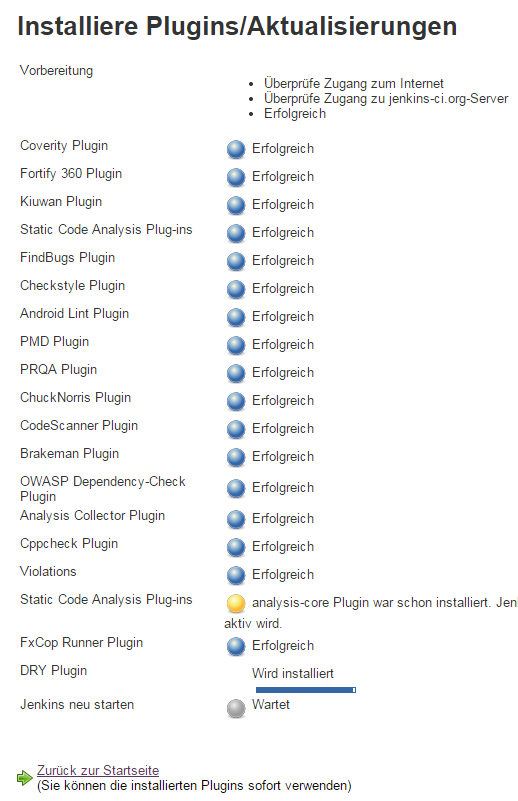
\includegraphics[width=1\linewidth]{img/jenkins-code-analysis-plugins.png}
%	\caption{Just a few used Jenkins plugins for static code analysis}
%	\label{fig:jenkins-plugins}
%\end{figure}


\subsection{Teamcity}
\label{subsec:static_code_analysis_teamcity}
Like Jenkins, Teamcity is a web application for continuous integration, published by the company Jetbrains\footnote{\href{https://www.jetbrains.com/teamcity/}{https://www.jetbrains.com/teamcity/}}. In contrast to Jenkins, its not open source, but freely available with a limitation of 20 build configurations.
Also it claims to be easier to use and configure than Jenkins.
It provides possibilities to run analyzers before or after the build process and to inspect resulting reports.
Furthermore it works together with static code analyzers in the commercial IntelliJ\footnote{\href{https://www.jetbrains.com/idea/}{https://www.jetbrains.com/idea/}} IDE from Jetbrains.

\begin{itemize}
	\item Installation: The Teamcity installation was a bit easier than Sonarqube because the database connection was configured in a wizard and similar it consists out of a webserver with webinterface (localhost:8111) and a database.
	
	\item Language support: All (since it is a highly customizable CI tool)
	
	\item Rule Management: The analyzers have to run externally and Teamcity will import the analysis results.
	Hence, it is much effort to configure and install different analyzers with different rulesets.
	
	\item Issue-Presentation: In the build details you can show issues in the Code Inspection tab, what present just the xml tree of the parsed reports, no filter options, no resolve options, no severity levels.
	
	\item Positive: Better user interface than Jenkins. With installed IDE plugin, you can jump to issue source-code directly in the IDE. 
	
	\item Negative: Hard to configure the external pmd and findbugs reports. Visualization of issues very limited. Two different inspections can not be processed during one build (skipped PMD report)
	
\end{itemize}





\section{Static code analysis in Code Quality Management}
\label{sec:static_code_analysis_code_quality_management}

\todo[inline]{Lofti: CQM although interesting, it is related to a different problem, unless you describe the connection to CI well.}

Code quality management (CQM) is the practice of monitoring and controlling the quality of code with different metrics and activities.
Static code analysis is a method of gaining measurements that can be used for CQM. Therefore, CQM tools can benefit at lot by a integration of static code analysis into a common build system.

\todo[inline]{quality management advantages and disadvantages}

\subsection{SonarQube}
\label{subsec:sonarqube}
SonarQube\footnote{\href{http://www.sonarqube.org/}{http://www.sonarqube.org/}} is an open source project, implemented as web application within its own webserver, with the aim to analyze and manage the quality of source code. 
Besides analysis against common coding guidelines, like duplicate code, missing comments and potential bugs, it also checks for several security issues (e.g. from the OWSASP Top 10 list).
Therefore it provides a central place to manage intuitively analysis rules from different analyzer extensions.
The main difference to CI tools, is the feature to manage the found issues.
Over plugins it is possible to extend the analysis scope to over 20 programming languages.


\begin{itemize}
\item Installation: SonarQube consists out of 3 parts: the local webserver (localhost:9000), a database to load and store analysis results and the sonarqube runner, which analyses the code specified in a project property file.

\item Language support: Java and other languages available as plugins

\item Rule Management: Very intuitive and easy to configure rules for so called quality profiles. Very interesting, that you can manage the rules of all analyzer plugins in one menu. It comes already with default sonarqube rules with different severity levels, detailed descriptions in different categories. Also including security relevant rules e.g. from OWASPTop10 and CWEs. One can compose a static analysis out of those rules including rules from plugins like FindBugs and PMD.

\item Issue-Presentation: Dashboard as starting point presents overview very well with different informative metrics, mostly for code quality and presents the number of issues of the different severity levels.
In the menu issues and issue-drilldown one can sort the issue list, search for issues matching to specific rules and get more information to the issue and most important where the issue is located in the code.

\item Positive: Good overview over issues, fast analysis, good rule management, good issue management with assigning issues to users etc.

\item Negative: In Rule-Management one can filter rules by tags and categories (bugs, security bugs), but you can not use those filters in the issue management. This leads to a big list of issues where you cant distinguish e.g. between a unused code and security issue.
 
\end{itemize}






%We subdivide our evaluations by programming language because the analyzers and their main purpose differs heavily in respect to their target language.

%\section{C/C++}

\subsection{Cppcheck}
\textit{Cppcheck} is a very powerful analyzer for C and C++ which can find a lot different code issues. For example it tries to find out-of-bounds accesses, memory leaks or warn if obsolete or unsafe functions are used. Its main goal is to avoid false positives.

Cppcheck is easy to use and can be integrated in an continuous life cycle with very little effort.
Listing \ref{lst:cppcheck} shows how to run a Cppcheck analysis on C/C++ project. When you use this command, Cppcheck will run with 4 threads (\texttt{-j 4}), does all analysis it supports (\texttt{--enable=all}) and writes the results as xml file on disk after it examined any C/C++ file in the current folder and any folder below that (recursively).

\begin{lstlisting}[caption={Bash command to run Cppcheck},label={lst:cppcheck}]
$ cppcheck -j 4 --enable=all \
	--xml --xml-version=2 . \
	2> cppcheck.xml
\end{lstlisting}


\subsubsection{Cppcheck \& Jenkins}
There exists a dedicated \href{https://wiki.jenkins-ci.org/display/JENKINS/Cppcheck+Plugin}{Jenkins plugin for Cppcheck}. This plugin does not include the Cppcheck analysis. This has to be performed as a build step which produces a XML-file containing the analysis results. The plugin will then, as a post-build task, read the XML-file and display the contents in a processed manner.

\subsubsection{Cppcheck \& SonarQube}






\section{Evaluation}
\label{sec:evaluation}
We decided to make a qualitative evaluation, with usability inspection heuristics described in the book Information Visualization by Kerren et al. \cite{InformationVisualizationBook}.
From the work of Hollingsed et al. on 15 years of usability inspection evaluation \cite{15yearsUsabilityEvaluation}, we derived the best method would be a combination of a cognitive walk-through, combined with the usability heuristic evaluation defined by Nielsen \cite{Nielsen:UsabilityInspectionMethods}.
This wide-used, informal, very cost efficient and effective method is proven to find with a appropriate skilled evaluator team 55 - 90\% of all usability problems.


The usability inspection over heuristic evaluation method uses a small group of usability experts, who evaluate a
user interface using a set of guidelines and noting the severity of
each usability problem and where it exists. 
We combine it with a cognitive walk-though, in the way, that three experts go through the tools with a cognitive expected path in context of applying static code analysis with an additional usability guidelines list for every stage.


We identified four stages of our walk-through and evaluate several usability guidelines in each stage:


\subsection{Prepare analysis}
\begin{itemize}
	\item \textit{Is the tool easy and intuitive to configure?} \\
	In this category, we appraise how complicated it was, to set the continuous integration environment up and create a test project with our test source.
	
	\item \textit{Is it possible to add external analyzers?} \\
	This is a very useful feature, maybe even elementary. Not being able to add external analyzers means that only the included analyzers can be used.
	
	\item \textit{Is it possible to configure the analyzers?} \\
	Configuring static code analyzers is mandatory. For example, there is a huge trade of between accuracy and speed. Accurate analysis can result in very high computational costs. Keep in mind that the anaysis is supposed to run for each commit. If an analyzer run takes hours, this would not be practical anymore.
	
	\item \textit{Is it possible to view the rules?} \\
	This question targets the openness of the used static analysers. It can be very helpful to be able to view all supported rules if you want, for instance, check if a specific feature is checked or not. Additionally, viewing the rules can help to understand why an issue was reported and how the code can be improved.
	
	\item \textit{Is it possible to choose, add, edit, delete rules?} \\
	This is related to the previous question, but goes a little further. Imaging you got ascertain that at specific flaw is not detected by a static code analyser. In case, the analyser supports the editing of the used ruleset, you can simply add a custom rule or edit an existing one.
	
	Choosing (selecting) only a subset of all existing rules can result in a faster analyser run which can come in very handy if frequent analyzis should be performed, e.g. at each commit and thereby multiple times a day.
\end{itemize}


\subsection{Run analysis}
\begin{itemize}
	\item \textit{Is it easy and intuitive to start the analysis?} \\
	How much effort is required to manually start an analysis? Is this even possible or are only automated analysis supported? Furthermore, starting an anylsis can be easy as a click on a website or hard like a manuell invokation of a specific command on the source code folder on some server.
	
	\item \textit{Is it possible to following the analysis progress?} \\
	This can be useful if an anylsis takes some time and the process cannot be determinded in a different way. Also, the analyser output can be helpful for debugging purposes.
\end{itemize}


\subsection{Evaluate analysis results}
\begin{itemize}
	\item \textit{Is there an issue overview with severity levels?} \\
	\item \textit{Is it possible to view an issue trend/history?} \\
	\item \textit{Is there a mapping from issue to source code position?} \\
	\item \textit{Is there a description for every issue?} \\
	\item \textit{Is the issue description easy to understand with solution suggestions?} \\
	\item \textit{Is there a possibility to filter issues? (severity, category, tag, ...)} \\
\end{itemize}


\subsection{Manage analysis results}
\begin{itemize}
	\item \textit{Is it possible to assign issues to developers?} \\
	\item \textit{Is is possible to edit issue status? (Resolved, False positive, ...)} \\
\end{itemize}



\subsection{Eclipse}
\label{subsec:evaluation_eclipse}

\subsection{Jenkins}
\label{subsec:evaluation_jenkins}
Jenkins itself has no static code analysis included but a major feature of Jenkins is its extensibility. Including a code analysis step in a build process is simple as adding a \textit{build step}. The analysers configuration can be passed by command line options or via a configuration file, depending on the used analyser.

Result visualization is done by free plugins. In general, the analyser creates a result file that is written to a specific location. After the build is done, the relevant plugins check the project root for those result files and parse their content. Therefore, the way the results are shown depends largely on the quality of the used plugin.


\subsection{Teamcity}
\label{subsec:evaluation_teamcity}

\subsection{SonarQube}
\label{subsec:evaluation_sonarqube}


\subsection{Comparison}
\label{subsec:comparation}

\begin{figure*}[t]
	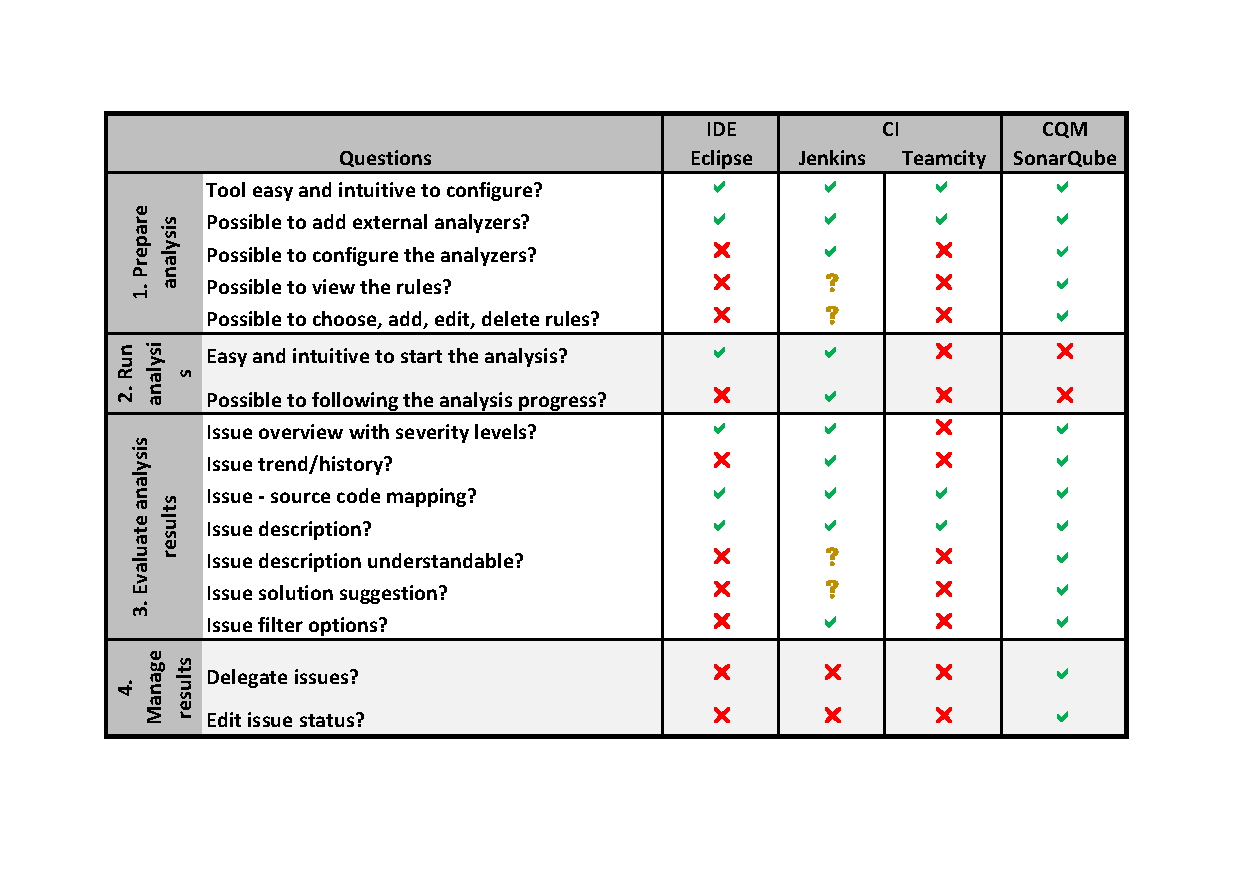
\includegraphics[width=\textwidth]{img/comparation}
	\caption{Comparison Matrix.}
	\label{fig:comparison_matrix}
\end{figure*}


\todo[inline]{Describe the final analysis results (matrix)}

\section{Conclusion}
\label{sec:conclusion}
\begin{itemize}
	%\item Conclusion about how input validation is done in frameworks, what can be better ...
	\item Its really not that easy to find the right static code analyzer for your project with a specific programming language. There are lots of open source tools, but very old and just supported by Jenkins over hacks.
	\item static code analyzer need to be customized to find special problems (like Java Vulnerabilities)
	\item Is it better to integrate static analysis in Jenkins or in IDE or in Code Quality Management tools?
	\item Is reporting in Jenkins useable? No...just in combination with code quality management tools like SonarQube, Coverity, ... and the analysis in those tools can be triggered in CI tools, but it is much effort to configure.
	\item Future work: Using many tools is basically a good idea, because more tools find potentially more vulnerabilities. A future approach would be to implement a tool that can filter all the generated reports. Thereby duplicate vulnerabilities findings can be merged and false positives can be reduced.
\end{itemize}



\bibliographystyle{IEEEtran}
% argument is your BibTeX string definitions and bibliography database(s)
\bibliography{references}

\end{document}


